\documentclass[12pt, french]{article}

\usepackage{fancyhdr, fancybox, lastpage}
\usepackage[most]{tcolorbox}
\usepackage[a4paper, margin={0.3in, .75in}]{geometry}
\usepackage[siunitx, RPvoltages]{circuitikz}
\usepackage{wrapfig}
\pagestyle{fancy}
\renewcommand\headrulewidth{1pt}
\renewcommand\footrulewidth{1pt}
\fancyhf{}
\rhead{ \em{Zakaria Haouzan}}
\lhead[C]{\em{1ére année baccalauréat Sciences Mathématiques}}
\chead[C]{}
\rfoot[C]{}
\lfoot[R]{}
\cfoot[]{\em{Page \thepage / \pageref{LastPage}}}


\newtcolorbox{Box2}[2][]{
                lower separated=false,
                colback=white,
colframe=white!20!black,fonttitle=\bfseries,
colbacktitle=white!30!gray,
coltitle=black,
enhanced,
attach boxed title to top left={yshift=-0.1in,xshift=0.15in},
title=#2,#1}


\begin{document}
\begin{center}
   \shadowbox {\bf{Comportement global d’un circuit }}
\end{center}


%%_________________________Exercice ! :"_________________________Exercice
   \begin{Box2}{Exercice 1 : l’énergie électrique et rondement }

      L’équation de la caractéristique traduisant la loi d’ohm aux bornes d’un générateur est :$ U_{PN} = 1.5 - 2I$

      1. Déterminer la f.é.m. E et la résistance interne r de ce générateur.

      2. On effectue ensuite une étude énergétique dans le cas où le générateur fonctionne durant 10 minutes. La tension à ses bornes est 1V.

      2.1. Calculer l’énergie dissipée par effet joule.

      2.2. Calculer l’énergie fournie par le générateur au reste du circuit.

      2.3. Calculée l’énergie électrique générée.

      2.4. Calculer le rondement de ce générateur, conclure.
   \end{Box2}


%%_________________________Exercice !2 :"_________________________Exercice
\begin{Box2}{Exercice 2 :le point de fonctionnement du circuit. }
Un circuit électrique comporte un générateur (E = 6V; r = 2$\Omega$ )et un électrolyseur
(E' = 2,4V ; r' = 10 $\Omega$ ).

1. Déterminer le point de fonctionnement du circuit.

2. Calculer la puissance électrique engendrée par le générateur, la puissance que peut
recevoir l’électrolyseur et la puissance utile transformée en réactions chimiques.

3. Calculer le rendement du générateur et aussi de l’électrolyseur. Calculer le rendement
du circuit.
\end{Box2}

%%_________________________Exercice ! 3:"_________________________Exercice
\begin{Box2}{Exercice 3 :  Le moteur (M) électrique d’un treuil }

   Le moteur (M) électrique d’un treuil est alimenté par une batterie d’accumulateurs. Cette dernière est considérée comme un générateur de f.é.m. 144 V et de résistance interne 0,1$\Omega$.

1.a. Calculer l’énergie électrique transférée par la batterie au moteur M du treuil si ce dernier est traversé par un courant d’intensité 35 A durant 3 s.

1.b. En déduire le rondement de la batterie.

2. Le treuil soulève, à vitesse constante, un bloc de béton de 630 kg, d’une hauteur de 1,7 m en 3s . Sachant que l’intensité du courant électrique qui traverse le moteur est 35A.

2.a  Calculer la valeur de l’énergie convertie par le moteur en énergie mécanique.
On donne : $g = 9,8 N/kg$

2.b. Quel est le rondement du moteur ?

2.c. En déduire La f.é.m. E’ du moteur M.

3. La résistance interne du moteur est r = 0,4 $\Omega$.

3.a. Calculer l’énergie dissipée par effet joule.
3.b. Le principe de conservation de l’énergie est-il vérifié au niveau du moteur ? Interpréter ce
résultat.
\end{Box2}

\begin{Box2}{Exercice 4 : Schéma énergétique}
   Un générateur de f.é.m. E = 33V débite un courant d’intensité I = 11A lorsqu’il est connecté à un conducteur
ohmique de résistance R = 2,5$\Omega$. Calculer :

   1. la puissance dissipée par effet Joule dans le conducteur ohmique,

   2. la puissance totale disponible dans le générateur,

   3. la puissance dissipée par effet Joule dans le générateur,

   4. la résistance interne du générateur.

   5. Faire un schéma énergétique montrant les transferts d’énergie s’effectuant au niveau de chaque dipôle de
circuit .
\end{Box2}
\begin{center}
   \Large{ \em{Exercices Supplémentaires}}
\end{center}


%%_________________________Exercice 4 : _________________________Exercice
\begin{Box2}{Exercice 5 : les paramètres d’une pile }
\begin{wrapfigure}{r}{0.3\textwidth}
  \begin{center}
     \vspace{-0.5cm}
    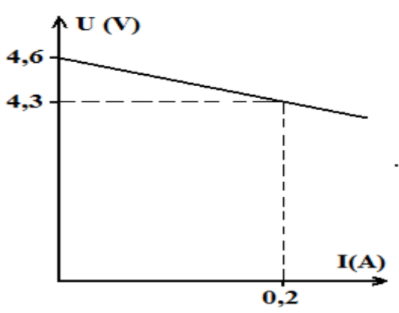
\includegraphics[width=0.3\textwidth]{./img/carcateristique_generateur.png}
  \end{center}
\end{wrapfigure}
  
   Au cours d’une séance de travaux pratiques, on détermine les paramètres (E, r) d’une pile de 4,5V en traçant sa
caractéristique intensité - tension.

1. Proposer un montage électrique pour tracer cette caractéristique. On dispose de la pile, d’une résistance variable (0-100$\Omega$ ; 0-2 A), de deux multimètres et d’un interrupteur.
Faites apparaître sur ce circuit les deux bornes de chaque multimètre, la flèche de la tension mesurée ainsi que
l’intensité du courant.

   On a la courbe suivantes.En déduire la force électromotrice E et la résistance interne r de cette pile. Justifier.

   2. Pour une tension U = 4,21 V, déterminer :
\\a. La puissance électrique fournit au circuit extérieur.
\\b. La puissance chimique transformée en puissance électrique.
\\c. La puissance dissipée sous forme d’effet Joule dans la pile.
3) Faire un schéma énergétique montrant les transferts d’énergie s’effectuant au niveau de la pile.
\end{Box2}
%\vspace{2cm}
%%_________________________Exercice 5 : _________________________Exercice
\begin{Box2}{Exercice 6 : bilan énergétique}
\begin{wrapfigure}{r}{0.4\textwidth}
  \begin{center}
     \vspace{-0.5cm}
    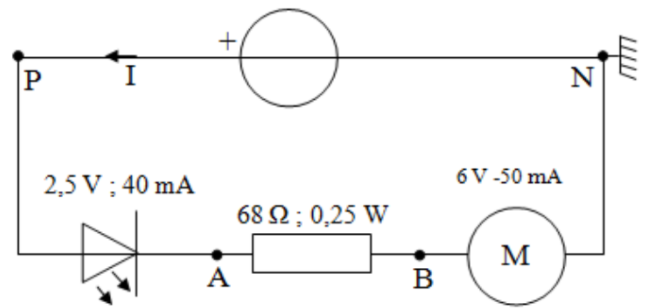
\includegraphics[width=0.4\textwidth]{./img/diode_circuit.png}
  \end{center}
\end{wrapfigure}
On réalise le circuit suivant :
   \\- $U_{PN}=12,16 V$
\\- $I=48 mA$
   \\- $U_{PA}=2,62 V$
   \\- $U_{AB}=3,28 V$
   \\- $U_{BN}=6,28 V$

   On règle le générateur sur 12 V continue

   1. Que signifient les valeurs indiquées au-dessus de chaque récepteur ?

   2. Flécher sur le schéma les tensions UPN, UPA, UAB et UBN. Mesurer chacune d’entre elle.

   3. Mesurer l’intensité du courant qui est débitée par le générateur.

   4. Que dire du courant qui circule dans les récepteurs ? Le vérifier par une mesure pour le moteur

   5. Exprimez puis calculer l’énergie électrique E (en J) fournie au circuit par le générateur pendant
1minute.

   6. Exprimez puis calculer les énergies électriques E1, E2, E3 reçues respectivement par la DEL, la
résistance et le moteur pendant cette même durée.

   7. Quelle est la relation littérale qui lie E, E1, E2, E3 ? La vérifier numériquement.

   8. En déduire, à partir de ce bilan énergétique, la relation entre UPN, UPA, UAB et UBN. Vérifier la relation numériquement.
\end{Box2}
%%_________________________Exercice 6 : _________________________Exercice
\end{document}
